\section{Signal yield}
\label{sec:yield}
Two steps of fit are performed to determine the prompt signal yield in each kinematic intervals,
which are both extended unbinned maximum likelihood fit.
The first step is performed on the invariant mass $M(\proton\Km\pip)$ distribution in the selected signal window.
Following previous analyses~\cite{LHCb-PAPER-2019-021,LHCb-PAPER-2022-007},
a Crystal Ball (CB) function\cite{Skwarnicki:1986xj} plusk
a Gaussian function is used to describe the signal shape,
where
\begin{equation}\label{eqn:mass_pdf}
    f\times \mathrm{CB} + (1-f)\times \mathrm{Guass}~,
\end{equation}
\begin{equation}\label{eqn:crystal_ball}
    f_{\mathrm{CB}}(x;M,\sigma,\alpha,n)=\left\{
        \begin{array}{l}
            \frac{\left(\frac{n}{|\alpha|}\right)^n e^{-\frac 1 2 \alpha^2}}{\left(\frac{n}{|\alpha|}-|\alpha|-\frac{x-M}{\sigma}\right)^n},\ \ \text{if }\frac{x-M}{\sigma}<-|\alpha|~, \\
            \exp\left(-\frac 1 2 \left(\frac{x-M}{\sigma}\right)^2\right),\ \  \text{if }\frac{x-M}{\sigma}\geq-|\alpha| ~.
        \end{array}
        \right.
\end{equation}
A linear function is used to describe the shape of background.
In this \PDF, $n$ of CB function is always fixed to 1 from physical constraint,
and CB and Gaussian function share a common mean value.
Due to limited statistics in some kinematic intervals,
fit results will be unstable or hard to converge if all parameters.
Thus, a global fit is performed to fix $\alpha$ in CB,
the ratio between width of Gaussian over that of CB $r_\mathrm{width}$,
and the fraction of the CB function $f$.
To ensure the stability of the fits, the mass fits are repeated with 50 times,
varying the initial values of all parameters randomly.
The fit result with the smallest minimal negative likelihood (NLL)
is chosen to be the final result.
Such {\it best} results for two rapidities are shown in Fig.~\ref{fig:global_fit}.
\begin{figure}[tb]
    \begin{center}
        \includegraphics[width=0.48\linewidth]{plots/Lc_mass_total1/mass_best}\put(-40,150){(a)}
        \includegraphics[width=0.48\linewidth]{plots/Lc_mass_total2/mass_best}\put(-40,150){(b)}
        \vspace*{-0.5cm}
    \end{center}
    \caption{\small
    Fit on kinematic-unbinned $M(\kaon\pion)$ distribution for Fwd (left) and Bwd (right) rapidities. }
    \label{fig:global_fit}
\end{figure}

This invariant mass fit is performed in the signal window around \Lc PDG mass $M(\Lc)\pm 50\mev$ as listed in Table \ref{tab:offline}.
Here, {\it best} fit results are also selected following the method above.
Two examples for Fwd and Bwd rapidities are shown in Fig.~\ref{fig:mass_fit},
and all results are summarized in Appendix~\ref{app:yields}.
\begin{figure}[tb]
    \begin{center}
        \includegraphics[width=0.48\linewidth]{plots/Lc_mass_fit_fix1/mass_2_2}\put(-40,150){(a)}
        \includegraphics[width=0.48\linewidth]{plots/Lc_mass_fit_fix2/mass_2_2}\put(-40,150){(b)}
        \vspace*{-0.5cm}
    \end{center}
    \caption{\small
    Fit on $M(\kaon\pion)$ distribution for Fwd ($4<\pt(\Lc)<5\gevc$ and $2.5<y^*<3.0$, left)
    and Bwd ($4<\pt(\Lc)<5\gevc$ and $-4.0<y^*<-3.5$, right) rapidities. }
    \label{fig:mass_fit}
\end{figure}

A second step of fit on the \logipchisq(\Lc) is performed to get prompt yields from total yields,
following previous analyses\cite{LHCb-PAPER-2018-021, LHCb-PAPER-2022-007}
Here $\chi^2_{\mathrm{IP}}$ is defined as the difference in the vertex-fit $\chi^2$
of a given PV reconstructed with and without the candidate under consideration.
which is approximate to the significance of IP significance $\mathrm{IP}/\sigma(\mathrm{IP})$.
So non-prompt \Lc baryons have larger IP than prompt ones due to the decay length of \B hadrons,
and the two different components can be distinguished with this parameter.
To suppress the background component, a \sPlot method~\cite{Pivk:200ty} is performed using the fit result from $M(\kaon \pion)$ fit.
So the \logipchisq~ distribution of weighted data contains only prompt \Lc component and non-prompt component.
The \PDF describing the shapes is a Bukin function~\cite{bukin2007fitting} as follows:
\begin{equation}
    \mathcal{P}(x;\mu,\sigma,\epsilon,\rho_L,\rho_R) =
    \begin{cases}
        \exp\! \left\{ \frac{ (x-x_1)\epsilon\sqrt{\epsilon^2+1}\sqrt{2\ln{2}} }{ \sigma\left(\sqrt{\epsilon^2+1}-\epsilon\right)^2\ln\left(\sqrt{\epsilon^2+1}+\epsilon\right) }
        + \rho_L\left(\frac{x-x_1}{\mu-x_1}\right)^2 - \ln{2} \right\} & x \leq x_1, \\
        \exp\! \left\{ - \left[ \frac{ \ln\left(1+2\epsilon\sqrt{\epsilon^2+1}\frac{x-\mu}{\sigma\sqrt{2\ln{2}}}\right) }
        { \ln\left(1+2\epsilon^2-2\epsilon\sqrt{\epsilon^2+1}\right) } \right ]^2 \times \ln{2} \right\} & x_1 < x < x_2, \\
        \exp\! \left\{ \frac{ (x-x_2)\epsilon\sqrt{\epsilon^2+1}\sqrt{2\ln{2}} }{ \sigma\left(\sqrt{\epsilon^2+1}-\epsilon\right)^2\ln\left(\sqrt{\epsilon^2+1}+\epsilon\right) }
        + \rho_R \left( \frac{x-x_2}{\mu-x_2} \right)^2 - \ln{2} \right\} & x \geq x_2.
    \end{cases}
\end{equation}
$$\tiny x_1 = \mu + \sigma \sqrt{2 \ln 2} \left( \frac{\epsilon}{\sqrt{\epsilon^2+1}} -1 \right),
x_2 = \mu + \sigma \sqrt{2 \ln 2} \left( \frac{\epsilon}{\sqrt{\epsilon^2+1}} +1 \right)~.  $$
It is a asymmetric gaussian function,
with $\epsilon$ discribing the asymmetry and two $\rho\mathrm{s}$
discrbing the left and right tail length.
For both configurations, $\rho_L$ and $\rho_R$ of prompt component are fixed
while $\epsilon$, $\rho_L$ and $\rho_R$ of non-prompt component are fixed,
all using simulation results of from-\bquark($\decay{\Lb}{\Lc\pim}$) simulation fit
as shown Fig.~\ref{fig:mc_prompt} and \ref{fig:mc_fromb}.
\begin{figure}[tb]
    \begin{center}
        \includegraphics[width=0.48\linewidth]{plots/Lc_ip_MC1/Bukin_mcp_best}\put(-40,150){(a)}
        \includegraphics[width=0.48\linewidth]{plots/Lc_ip_MC2/Bukin_mcp_best}\put(-40,150){(b)}
        \vspace*{-0.5cm}
    \end{center}
    \caption{\small
    Global fit on \logipchisq~ distribution of prompt \Lc simulation for Fwd (left) and Bwd (right) rapidities. }
    \label{fig:mc_prompt}
\end{figure}

\begin{figure}[tb]
    \begin{center}
        \includegraphics[width=0.48\linewidth]{plots/Lc_ip_MC1/Bukin_mcb_best}\put(-40,150){(a)}
        \includegraphics[width=0.48\linewidth]{plots/Lc_ip_MC2/Bukin_mcb_best}\put(-40,150){(b)}
        \vspace*{-0.5cm}
    \end{center}
    \caption{\small
    Global fit on \logipchisq~ distribution of from-$b$ \Lc simulation for Fwd (left) and Bwd (right) rapidities. }
    \label{fig:mc_fromb}
\end{figure}

From the fit of second step, the prompt \Lc yield yield in signal window \mbox{$[1815,1915]\mevcc \times [-5,5]$} can be directly obtained,
as summarized in Fig.~\ref{fig:prompt_yield}.
There may be some \Lc signals outside the window
so its effect is considered in the evaluation of selection efficiencies.
The fraction of prompt component is also given from as Fig.~\ref{fig:pfraction}.
It is however not multiplied with raw yield because their correlation should be
considered while calculating the uncertainty of prompt yield, which is of more difficulties.
%The numerical results of prompt \Dz yields and prompt \Dz fractions are included
%in Table \ref{tab:prompt_yield1}, \ref{tab:prompt_yield2}, \ref{tab:prompt_fraction1} and \ref{tab:prompt_fraction2}
%in Appendix \ref{app:yields}.

\begin{figure}[tb]
    \begin{center}
        \includegraphics[width=0.48\linewidth]{plots/Lc_Prompt1}\put(-40,150){(a)}
        \includegraphics[width=0.48\linewidth]{plots/Lc_Prompt2}\put(-40,150){(b)}
        \vspace*{-0.5cm}
    \end{center}
    \caption{\small
    Prompt yields obtained from \logipchisq ~fit for Fwd (left) and Bwd (right), statistical uncertainties only.}
    \label{fig:prompt_yield}
\end{figure}

\begin{figure}[tb]
    \begin{center}
        \includegraphics[width=0.48\linewidth]{plots/Lc_Fraction1}\put(-40,150){(a)}
        \includegraphics[width=0.48\linewidth]{plots/Lc_Fraction2}\put(-40,150){(b)}
        \vspace*{-0.5cm}
    \end{center}
    \caption{\small
    The fraction of prompt \Lc component from fit for Fwd (left) and Bwd (right), statistical uncertainties only.}
    \label{fig:pfraction}
\end{figure}
\clearpage
